\setchapterpreamble[u]{\margintoc}
\chapter{Գծային տարածությունների կառուցվածքը}
\labch{structure}

\emergencystretch 2em

\section{Գծային թաղանթ}

Ինչո՞ւ ենք գծային տարածությունների և ձևափոխությունների մասին խոսելիս առանձնահատուկ ուշադրություն դարձնում ձախում պատկեր\-ված երկու վեկտորներին, այլ ոչ թե ասենք՝ աջ կողմի երկու վեկտորներին։

\begin{figure}[h]
    \centering
    \subfloat{{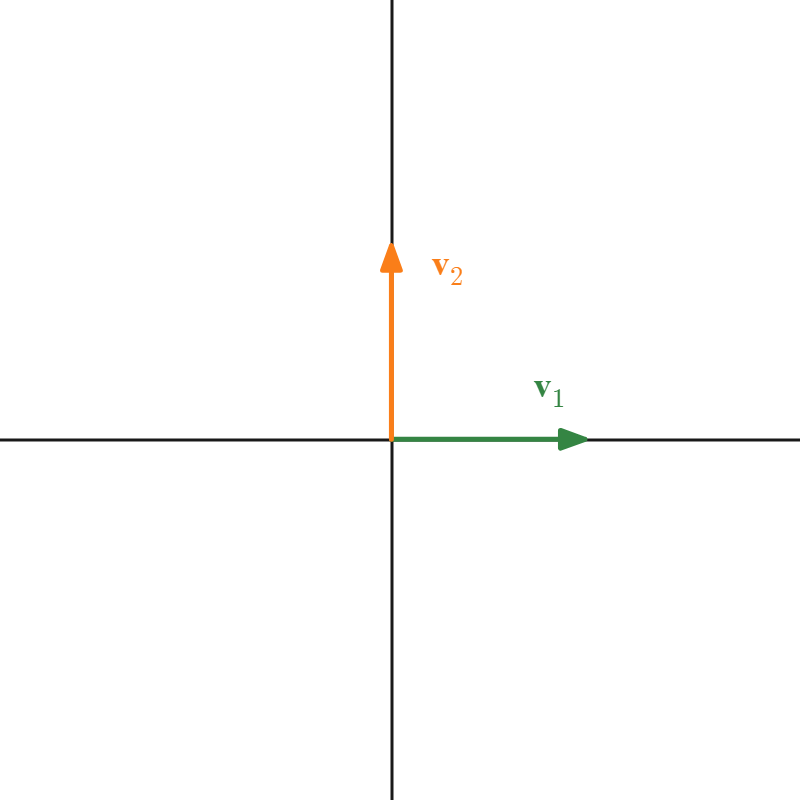
\includegraphics[width=0.4\linewidth]{chapters/chapter 4/two good vectors.png} }}%
    \qquad
    \subfloat{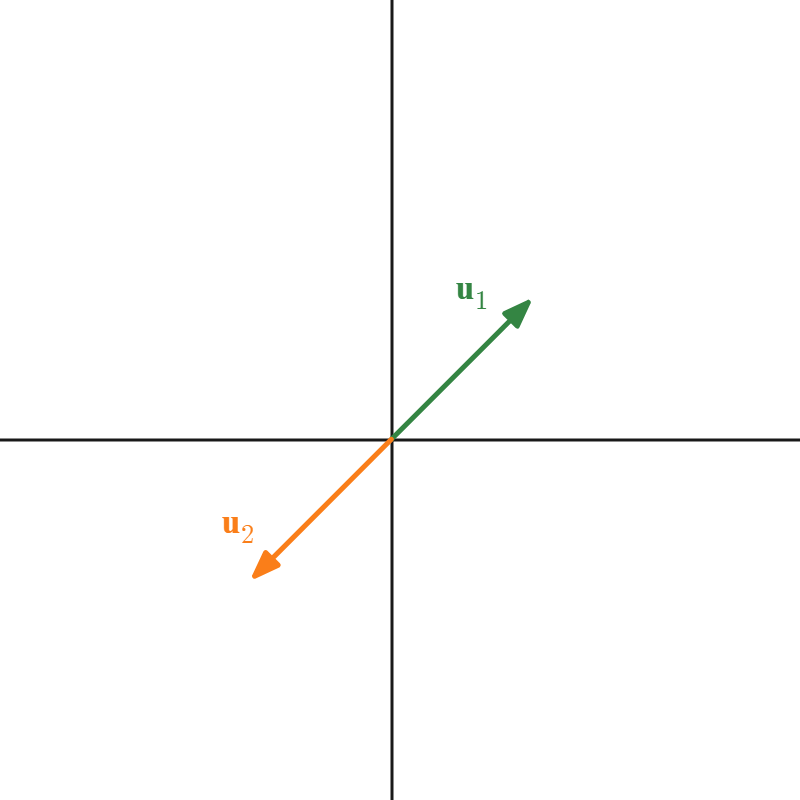
\includegraphics[width=0.4\linewidth]{chapters/chapter 4/two bad vectors.png}} %
\end{figure}

\textit{— Որովհետև ձախ կողմի երկու վեկտորներով կարելի է ստա\-նալ հարթության ցանկացած այլ վեկտոր,— }կասեք Դուք։

Իսկ ինչո՞ւ սահմանափակվել $\vv_1$, $\vv_2$-ով, ինչո՞ւ չնայել այս վեկտորներին՝

\begin{figure}[h]
    \centering
    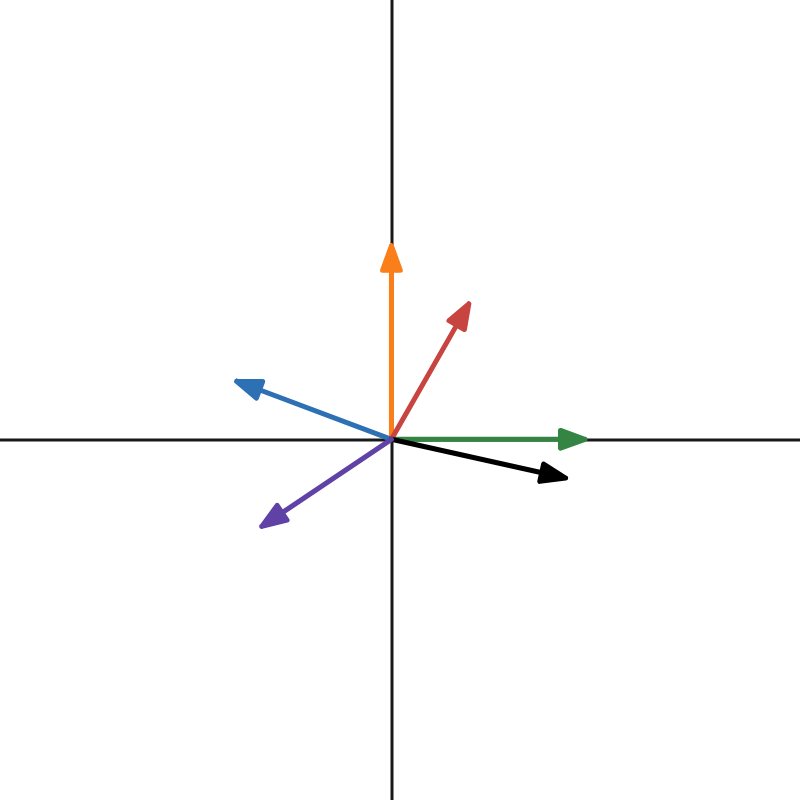
\includegraphics[width=0.4\linewidth]{chapters/chapter 4/too many vectors.png}
\end{figure}

Որովհետև սրանք արդեն չափից շատ են․ $\R^2$-ում բավարար է ունենալ երկու վեկտոր (առաջին նկարի նման), և դրանցով կարելի է ստանալ ցանկացած այլ վեկտոր։

Հստակ ձևակերպենք, թե ինչ նկատի ունենք «ցանկացած վեկտոր ստանալ» ասելով։ Եթե 
\[\vv_1=\begin{bmatrix}
    1 \\ 0
\end{bmatrix}, \qquad \vv_2=\begin{bmatrix}
    0 \\ 1
\end{bmatrix}
\]
ապա $\R^2$ տարածության յուրաքանչյուր $\vu$ վեկտոր կարող ենք գրել 
\[
\vu = (\text{ինչ-որ բան}) \cdot \vv_1 + 
(\text{ինչ-որ բան}) \cdot \vv_2
\]
տեսքով։ Օրինակ՝ $\begin{bmatrix}
    4 & -7
\end{bmatrix}$ վեկտորը կգրենք որպես՝
\[
\begin{bmatrix}
    4 \\ -7
\end{bmatrix}
= 4 \cdot \begin{bmatrix}
    1 \\ 0
\end{bmatrix}+ (-7) \cdot 
\begin{bmatrix}
    0 \\ 1
\end{bmatrix}
=  
4 \vv_1 - 7 \vv_2
\]

Այս դեպքում ասում ենք, որ $\begin{bmatrix}
    4 & -7
\end{bmatrix}$ վեկտորը $\vv_1$ և $\vv_2$ վեկտորների \textit{գծային զուգակցություն} է կամ պատկանում է $\vv_1$-ի և $\vv_2$-ի \textit{գծային թաղանթին։}

\begin{definition}
\[ 
c_1\mathbf{v}_1 + c_2\mathbf{v}_2 + \ldots + c_k\mathbf{v}_k 
\]
տեսքի ցանկացած արտահայտություն\marginnote{որտեղ $c_1$, $\ldots$, $c_k$ ցանկացած թվեր են} կանվանենք \(\mathbf{v}_1, \mathbf{v}_2, \ldots, \mathbf{v}_k\) վեկտորների \textbf{գծային զուգակցություն} (կոմբինացիա)։ 

$\vv_1$, $\vv_2$, $\dots$, $\vv_k$ վեկտորների բոլոր հնարավոր գծային զուգակցու\-թյուն\-ների բազմությունը կանվանենք այդ վեկտորների \textbf{գծային թաղանթ․}
\[
\operatorname{span}\{\vv_1, \vv_2, \ldots, \vv_k\} =    \{c_1\vv_1 + c_2\vv_2 + \ldots + c_k\vv_k \,\mid\, c_1, c_2, \ldots, c_k \in \mathbb{R}\}
\]
\end{definition}

\begin{figure}[h]
    \centering
    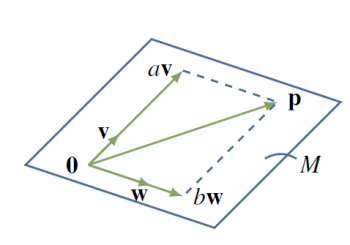
\includegraphics[width=0.5\linewidth]{chapters/chapter 4/span.png}
    \caption*{այստեղ $\mathbf{p}=a\vv+b\vw$}
\end{figure}

Երկրաչափորեն՝ $\vv_1$, $\dots$, $\vv_k$ վեկտորների գծային թաղանթը բոլոր այն վեկտորներն են, որոնք կարելի է ստանալ այդ վեկտորները ձգելով, սեղմելով և իրար գումարելով։ 

\begin{marginfigure}
% \centering
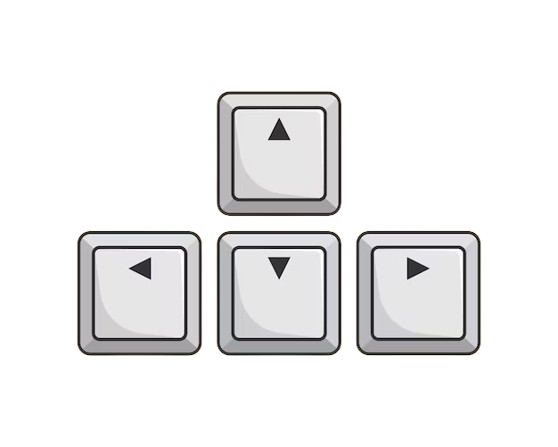
\includegraphics[width=0.8\linewidth]{chapters/chapter 4/arrow keys.png}
\end{marginfigure}

\question{Ո՞րն է $\leftarrow$, $\rightarrow$, $\uparrow$, $\downarrow$ կոճակների գծային թաղանթը։ Իսկ $\leftarrow$, $\rightarrow$ կոճակների՞նը։ Իսկ $\leftarrow$-ի՞նը։}

\begin{figure}[!h]
    \centering
    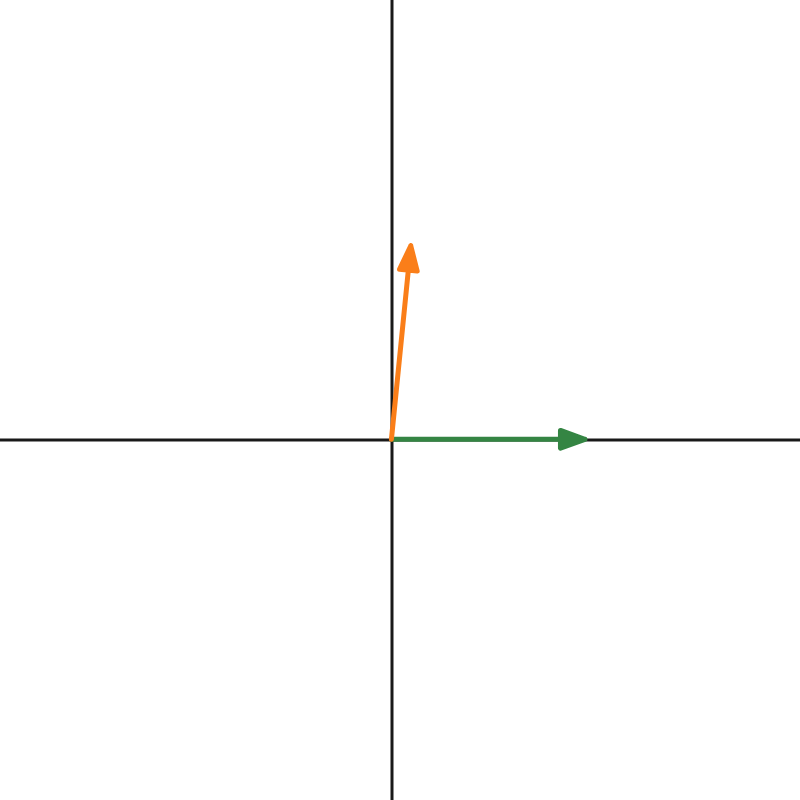
\includegraphics[width=0.4\linewidth]{chapters/chapter 4/span_1.png}
\end{figure}

\question{Հնարավո՞ր է $[4 \quad 3]$ վեկտորը արտահայտել $[1 \quad 0]$-ի և $[0.1 \quad 1]$-ի գծային զուգակցությունով։}

\begin{example}\label{2d_span}
\[
\begin{bmatrix}
    1 \\ 0
\end{bmatrix}
\qquad \text{և} \qquad 
\begin{bmatrix}
    0.1 \\ 1
\end{bmatrix}
\]
վեկտորների գծային թաղանթը կրկին $\R^2$-ն է։
\end{example}

\begin{figure}[!h]
    \centering
    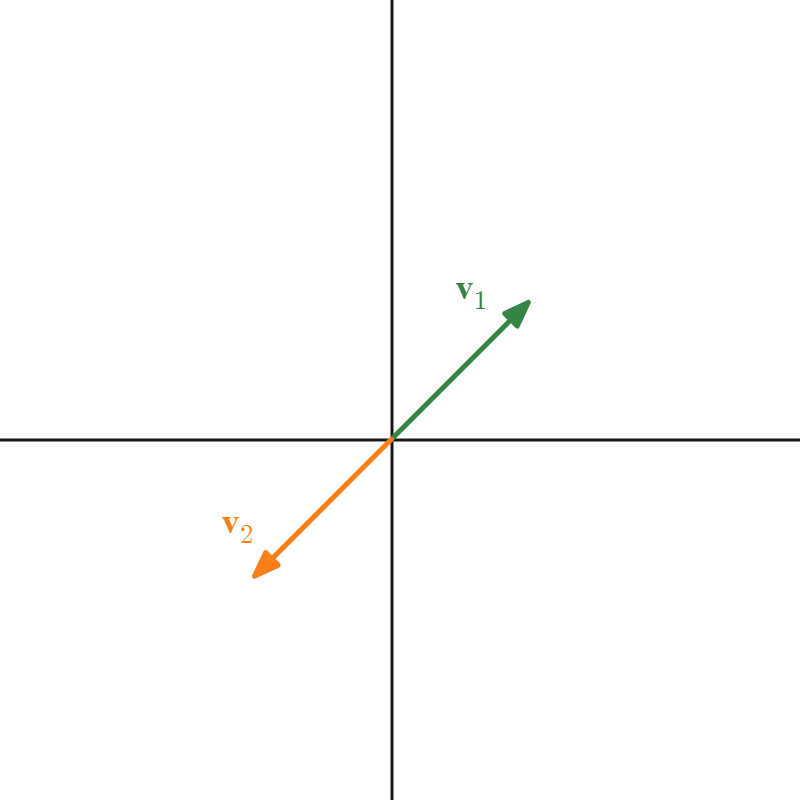
\includegraphics[width=0.4\linewidth]{chapters/chapter 4/span_2.png}
\end{figure}

\begin{example}\label{1d_span}
\[
\begin{bmatrix}
    1 \\ 1
\end{bmatrix}
\qquad \text{և} \qquad 
\begin{bmatrix}
    -1 \\ -1
\end{bmatrix}
\]
վեկտորների գծային թաղանթը $y=x$ ուղիղն է, քանի որ երկուսն էլ ընկած են այդ ուղղի վրա. հնարավոր չէ դրանք ձգելով-գումարելով ստանալ այդ ուղղից դուրս վեկտոր։
\end{example}

Ընդ որում, բավարար է վերցնել դրանցից միայն մեկը․ 


\begin{figure}[!h]
    \centering
    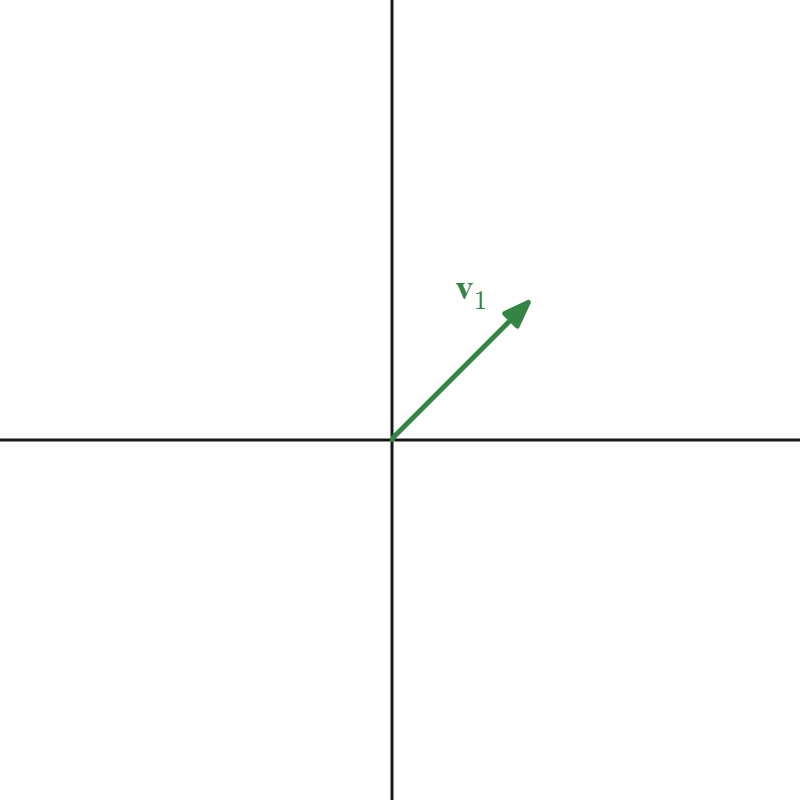
\includegraphics[width=0.4\linewidth]{chapters/chapter 4/span_3.png}
\end{figure}

\begin{example}
\[
\begin{bmatrix}
    1 \\ 1
\end{bmatrix}
\]
\marginnote{բազմապատկելով $-1$-ով՝ կստանանք $\vv_2$}վեկտորի գծային թաղանթը նույնպես $y=x$ ուղիղն է։
\end{example}

\question{Ո՞րն է $y=kx$ ուղղի վրա ընկած երկու վեկտորների  գծային թաղանթը։ Իսկ երեք վեկտորների՞։}

Նախորդ օրինակներում վեկտորների թաղանթը մի դեպքում ստացվեց հարթություն, մյուս դեպքում՝ ուղիղ։ Կարելի է ապացուցել, որ
\begin{theorem}
\marginnote{եթե վեկտորները $\R^n$-ում են, դրանց թաղանթը $\R^n$-ի ենթատարածություն է}Վեկտորների գծային թաղանթը գծային տարածու\-թյուն է։
\end{theorem}

\section{Գծորեն անկախություն}

Բայց ո՞րն է պատճառը, որ \hyperref[2d_span]{\color{OliveGreen} մի դեպքում} երկու վեկտորների գծային թաղանթը ամբողջ տարածությունն է, \hyperref[1d_span]{\color{OliveGreen} մեկ այլ դեպքում՝} ինչ-որ մի ուղիղ։ 

Տարբերությունն այն էր, որ երկրորդ դեպքում վեկտորները ընկած էին նույն ուղղի վրա, այսինքն հնարավոր էր դրանցից \textit{մեկը արտահայտել մյուսով։} Նման դեպքերում կասենք, որ վեկտորները \textit{գծորեն կախված} (կախյալ) են։

\begin{definition}
$\vv_1$, $\vv_2$, $\ldots$, $\vv_n$ վեկտորները կոչվում են \textbf{գծորեն անկախ,} եթե դրանցից ոչ մեկը հնարավոր չէ արտահայտել մյուսների գծային զուգակցության միջոցով։
\end{definition}

Եվ իհարկե, կասենք, որ վեկտորները \textbf{գծորեն կախված} են, եթե դրանցից որևէ մեկը (ասենք՝ $\vv_n$-ը) հնարավոր է արտահայտել մյուսներով՝
\[
\vv_n = c_1 \vv_1 + c_2 \vv_2 + \dots + c_{n-1}\vv_{n-1}
\]

\begin{figure}[h]
    \centering
    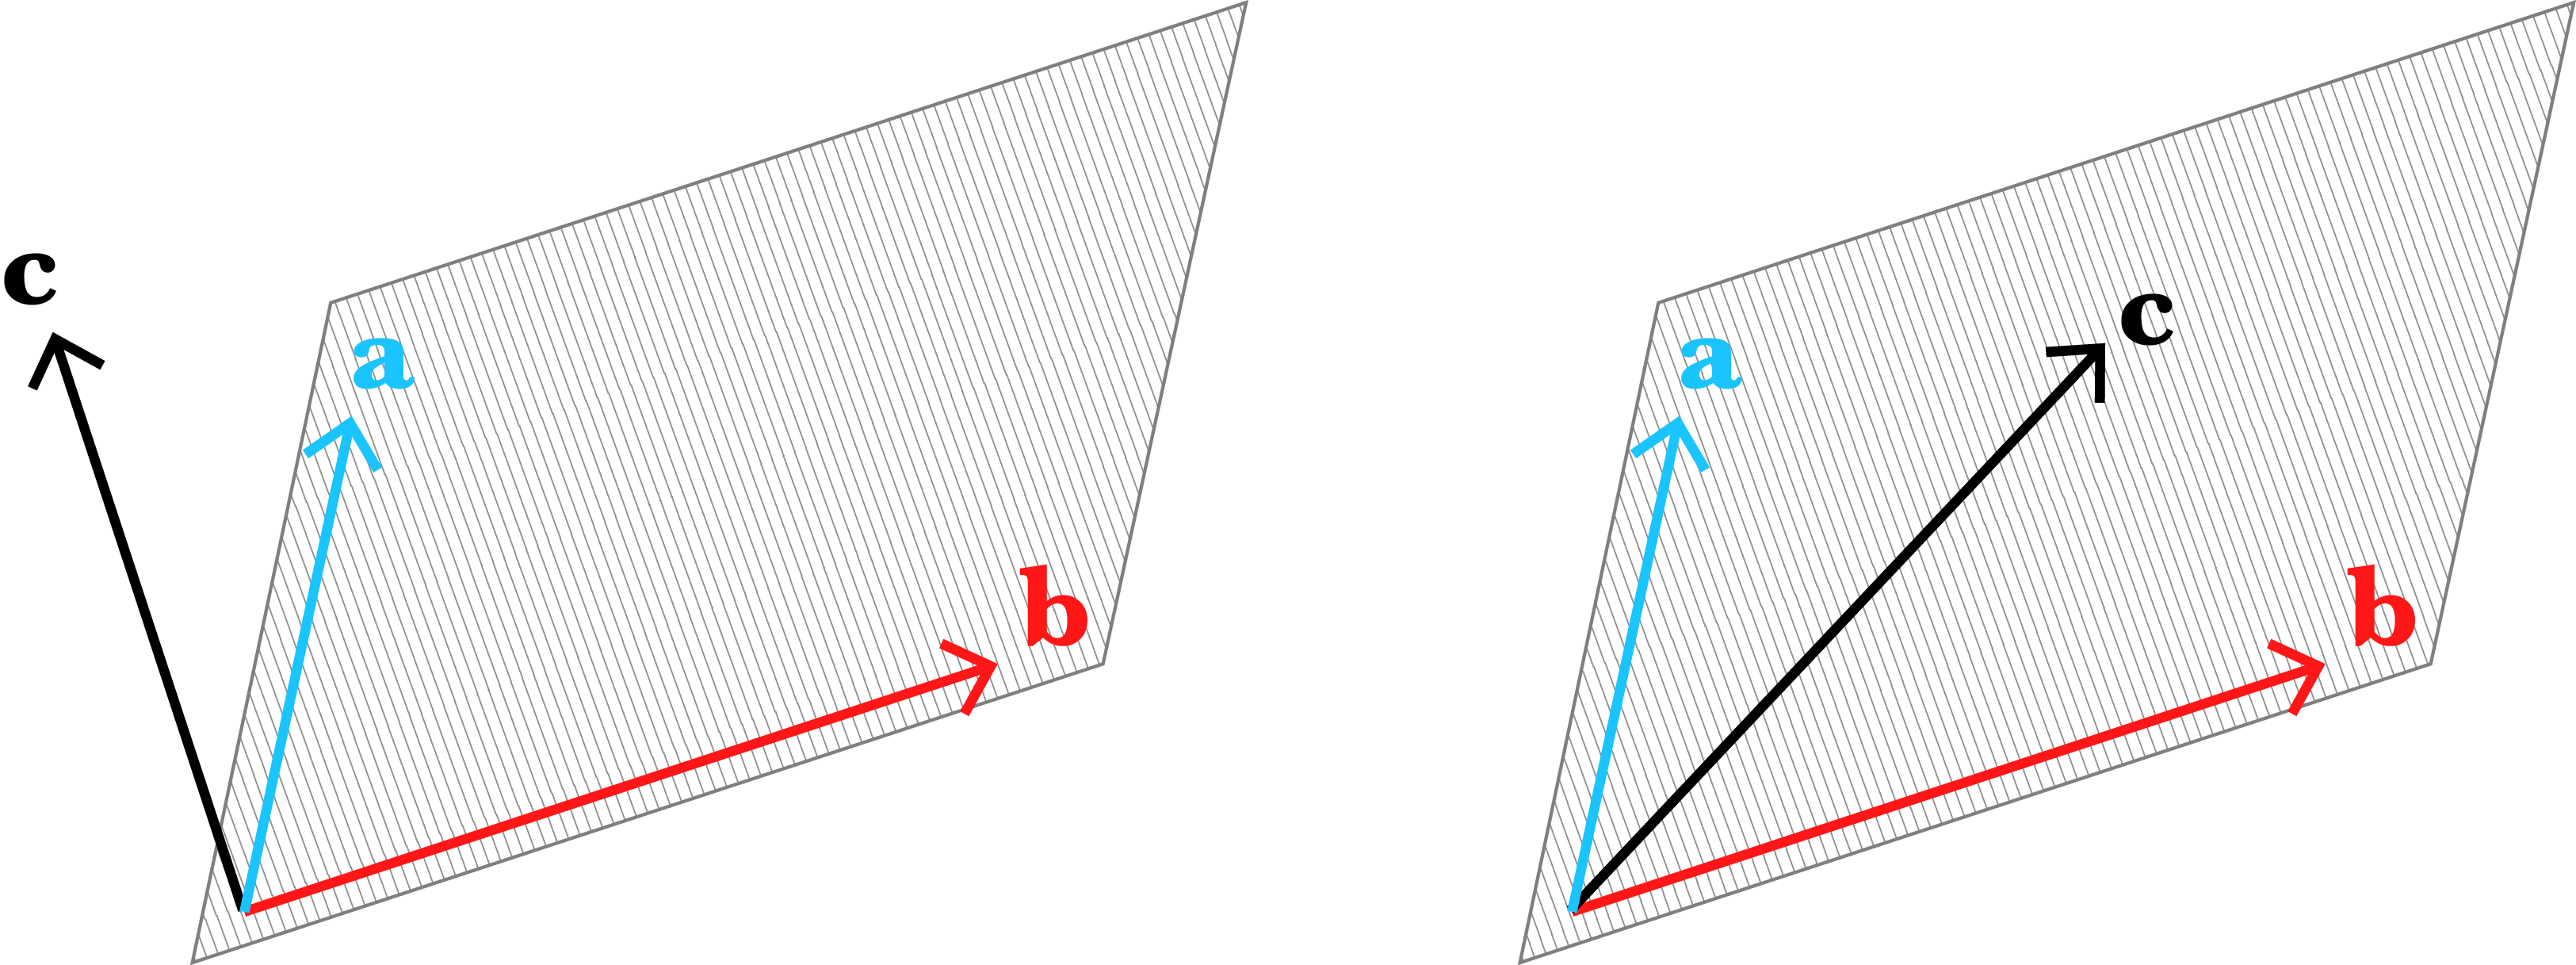
\includegraphics[width=0.85\linewidth]{chapters/chapter 4/linear-dependence-3d.png}
    \caption*{առաջին նկարում $\va$, $\vb$, $\vc$-ն գծորեն անկախ են, երկրորդում՝ ոչ}
\end{figure}


\question{Անցեք \href{https://www.desmos.com/calculator/gglf9fj10w}{հղումով} և խաղացեք $a$-ի ու $b$-ի հետ։ Ի՞նչ վեկտորներ եք ստանում։ Իսկ \href{https://www.desmos.com/calculator/1g2zq4exup}{այստե՞ղ}։}


Երկրաչափորեն,
\begin{itemize}
    \item երկու վեկտորներ գծորեն կախված են, եթե դրանք ընկած են միևնույն ուղղի վրա

    \item երեք վեկտորներ գծորեն կախված են, եթե դրանք ընկած են միևնույն հարթության մեջ
\end{itemize}
և այլն։

\question{$\vv_1$, $\vv_2$, $\vv_3$ վեկտորներից մեկը $\mathbf{0}$ է։ Կարո՞ղ են դրանք լինել գծորեն անկախ։}


Վեկտորների գծորեն անկախությունը ստուգելիս երբեմն հարմար է օգտվել հետևյալ թեորեմից (որը կարող եք ապացուցել):

\begin{theorem}
$\vv_1$, $\dots$, $\vv_n$ վեկտորները գծորեն անկախ այն և միայն այն դեպքում, եթե 
\[
\text{« } c_1\vv_1 + c_2\vv_2 + \ldots + c_n\vv_n = \mathbf{0} \text{ »}
\]
\marginnote{այսինքն՝ $0$-ից բացի ինչ թվեր էլ դնենք, գումարը $\mathbf{0}$ չի լինի}հավասարությունը տեղի ունի \textit{միմիայն} այն դեպքում, երբ $c_1 = c_2 = \ldots = c_n = 0$։
\end{theorem}


\section{Հենք}

Փաստորեն մեր
\[\vv_1=\begin{bmatrix}
    1\\0
\end{bmatrix}\qquad \text{ և }\qquad \vv_2=\begin{bmatrix}
    0\\1
\end{bmatrix}\] 
վեկտորները գծորեն անկախ են, և նրանց գծային թաղանթը ամբողջ $\R^2$-ն է։ 
Նման դեպքերում ասում ենք, որ $\vv_1$-ն ու $\vv_2$-ը կազմում են $\R^2$ տարածության \textit{հենք} կամ \textit{բազիս։}



\begin{definition}
$\vv_1$, $\vv_2$, $\dots$, $\vv_n$ վեկտորները կոչվում են $V$ գծային տարածության \textbf{հենք} (կամ \textbf{բազիս}), եթե
\begin{enumerate}
    \item $\vv_1$, $\vv_2$, $\dots$, $\vv_n$ գծորեն անկախ են, և
    
    \item $\vv_1$, $\vv_2$, $\dots$, $\vv_n$-ի գծային թաղանթը ամբողջ $V$-ն է։
\end{enumerate}
\end{definition}

Այսինքն՝ $V$-ի ցանկացած վեկտոր կարելի է արտահայտել $\vv_1$, $\dots$, $\vv_n$-ով, և դրանցից ոչ մեկն ավելորդ չէ․ եթե $\vv_i$-երից որևէ մեկը հեռացնենք, այն այլևս չի լինի հենք։

Ավելին, ցանկացած վեկտոր տվյալ հենքով կարելի է արտահայտել ուղիղ \textit{մեկ ձևով․} այսինքն օրինակ՝ $\begin{bmatrix}
    3 & 4
\end{bmatrix}$-ը $\vv_1=\begin{bmatrix}
    1 & 0
\end{bmatrix}$-ով ու $\vv_2=\begin{bmatrix}
    0 & 1
\end{bmatrix}$-ով արտահայտելու միակ ձևն է՝ $3\cdot \vv_1+4\cdot\vv_2$։

\begin{example}
\begin{marginfigure}
\centering
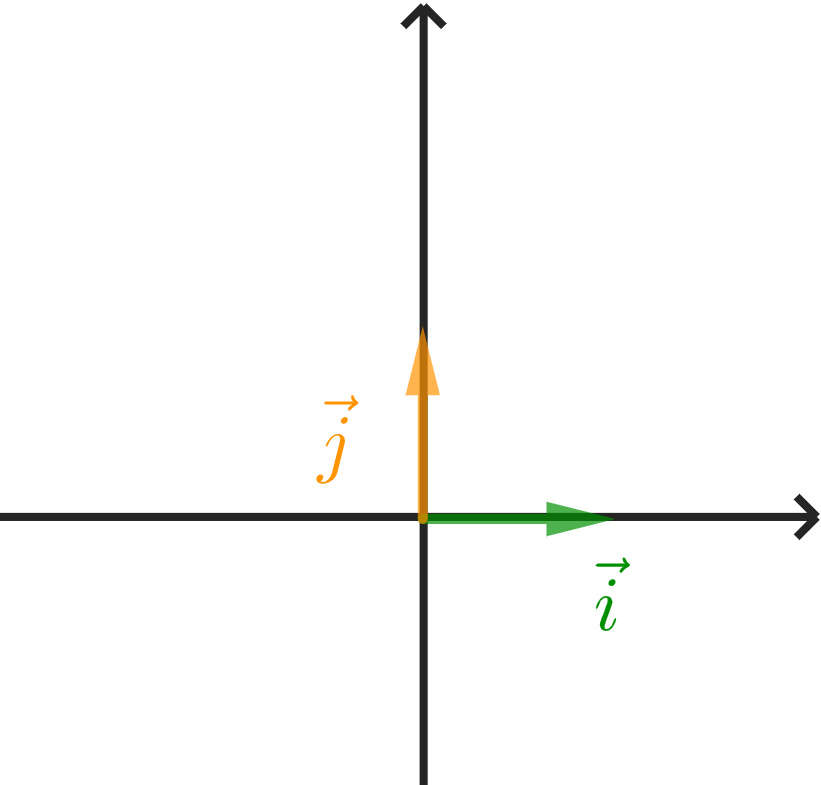
\includegraphics[width=0.6\textwidth, keepaspectratio]{chapters/chapter 4/ij basis.png}
\end{marginfigure}
\[
\mathbf{e}_1 = \begin{bmatrix} 1 \\ 0 \end{bmatrix}, \qquad \mathbf{e}_2 = \begin{bmatrix} 0 \\ 1 \end{bmatrix}
\]
վեկտորները $\mathbb{R}^2$-ի համար կազմում են հենք (կոչվում է $\R^2$-ի \textit{ստանդարտ հենք})։ Այս երկու վեկտորները հաճախ նշանակում են նաև $\hat{i}$, $\hat{j}$-ով։
\end{example}

\begin{example}
\begin{marginfigure}
\centering
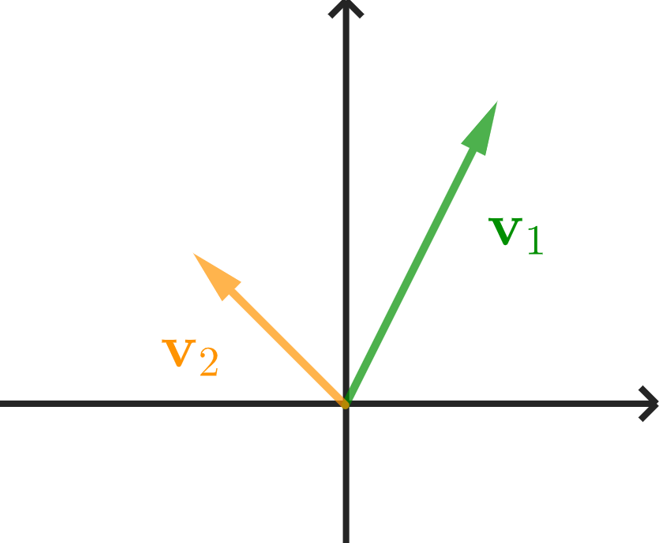
\includegraphics[width=0.6\textwidth, keepaspectratio]{chapters/chapter 4/v1v2 basis.png}
\end{marginfigure}
\[
\vv_1 = \begin{bmatrix} 1 \\ 2 \end{bmatrix}, \qquad \vv_2 = \begin{bmatrix} -1 \\ 1 \end{bmatrix}
\]
վեկտորները նույնպես $\mathbb{R}^2$-ի համար կազմում են հենք, քանի որ դրանք գծորեն անկախ են (ընկած չեն նույն ուղղի վրա), և դրանց թաղանթը $\R^2$-ն է։
\end{example}
  
\begin{example}
\begin{marginfigure}
\centering
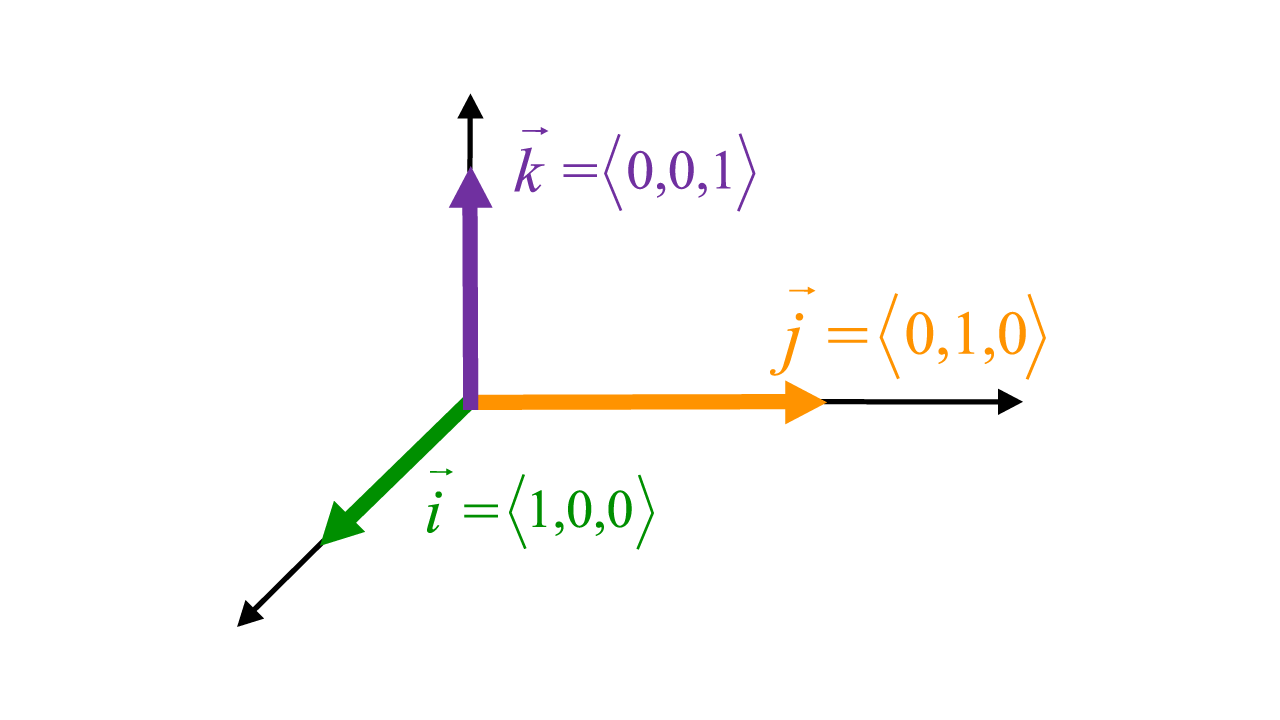
\includegraphics[width=\textwidth, keepaspectratio]{chapters/chapter 4/ijk basis.png}
\end{marginfigure}
\[
\mathbf{e}_1 = \begin{bmatrix} 1 \\ 0 \\ 0 \end{bmatrix}, \qquad \mathbf{e}_2 = \begin{bmatrix} 0 \\ 1 \\ 0 \end{bmatrix}, \qquad \mathbf{e}_3 = \begin{bmatrix} 0 \\ 0 \\ 1 \end{bmatrix}
\]
վեկտորները $\R^3$-ի համար կազմում են հենք ($\R^3$-ի \textit{ստանդարտ հենք}), նշանակվում են նաև՝ $\hat{i}$, $\hat{j}$, $\hat{k}$։
\end{example}

\question{Քանի՞ հենք ունի $\R^2$ տարածությունը։ Իսկ $\R^3$-ը՞։}


\begin{example}
\marginnote[*+2]{չափից դուրս շատ}\[
\vv_1 = \begin{bmatrix} 0 \\ 1 \end{bmatrix}, \qquad 
\vv_2 = \begin{bmatrix} 1 \\ 1 \end{bmatrix}, \qquad 
\vv_3 = \begin{bmatrix} 1 \\ 0 \end{bmatrix}
\]
վեկտորները $\R^2$-ի հենք չեն, քանի որ դրանք գծորեն կախված են։

\marginnote[*+2]{չափից դուրս քիչ}\[
\vv_1 = \begin{bmatrix} 1 \\ 0 \\ 0 \end{bmatrix}, \qquad 
\vv_2 = \begin{bmatrix} 0 \\ 1 \\ 0 \end{bmatrix} 
\]
վեկտորները $\R^3$-ի հենք չեն, քանի որ դրանց թաղանթն ամբողջ $\R^3$-ը չէ (այլ ինչ-որ մի հարթություն)։

\marginnote[*+2]{չափից դուրս անկապ}\[
\vv_1 = \begin{bmatrix} 1 \\ 0 \end{bmatrix}, \qquad 
\vv_2 = \begin{bmatrix} 4 \\ 0 \end{bmatrix} 
\]
վեկտորները $\R^2$-ի հենք չեն, քանի որ դրանք ոչ գծորեն անկախ են, ոչ էլ դրանց թաղանթն է $\R^2$-ը։
\end{example}

\begin{marginfigure}
    \centering
    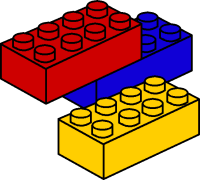
\includegraphics[width=0.6\linewidth]{chapters/chapter 4/lego.png}
    \caption*{հենքի վեկտորները մեր լեգոներն են, որոն\-ցով կառուցում ենք տարածությունը}
\end{marginfigure}

Ինչպես նկատում ենք, ամեն գծային տարածություն ունի բազմաթիվ տարբեր հենքեր (այլ ոչ թե միայն մեկը), բայց այդ բոլոր հենքերը բաղկացած են \textit{միևնույն թվով վեկտորներից։} Այդ թիվը կոչվում է տարածության \textit{չափողականություն։}


\begin{definition}
$V$ գծային տարածության հենքերից յուրաքան\-չյու\-րում եղած վեկտորների թիվը կանվանենք $V$-ի \textbf{չափողա\-կա\-նու\-թյուն} և կնշանակենք $\dim V$-ով։
\end{definition}

Եթե օրինակ $\R^2$-ում վերցնեք նույն ուղղի վրա չընկած երկու վեկտոր (կամ $\R^3$-ում նույն հարթության մեջ չընկած երեք վեկտոր), ապա ինչ վեկտորներ էլ վերցնեք, դրանք կկազմեն հենք։ Ավելի ընդհանուր՝ $\R^n$-ում ցանկացած $n$ հատ գծորեն անկախ վեկտոր կազմում են $\R^n$-ի հենք, հետևաբար՝
\begin{itemize}
    \item $\R^1$-ի չափողականությունը $1$ է
    \item $\R^2$-ի չափողականությունը $2$ է
    \item $\R^3$-ի չափողականությունը $3$ է
    \item $\dots$
    \item $\R^n$-ի չափողականությունը $n$ է
    \item ցանկացած ուղղի չափողականություն $1$ է
    \item ցանկացած հարթության չափողականություն $2$ է
    \item և այլն
\end{itemize}

Երկրաչափորեն չափողականությունը ցույց է տալիս, թե որքան մեծ է տարածությունը, թե ամենաշատը քանի գծորեն անկախ վեկտորներ է կարելի վերցնել այդ տարածության մեջ։

\question{Կարո՞ղ եք գտնել մատրիցներ, որոնք $2\times 2$ չափանի մատ\-րից\-ների տարածության մեջ կազմում են հենք։ Որքա՞ն է $\dim \R^{2 \times 2}$-ը։}


\section{Հենքի փոփոխություն}

Վերադառնանք գծային ձևափոխություններին։ Ընդհանուր առմամբ՝ յուրաքանչյուր մատրից տարածությունը որոշ չափով ձգում, սեղմում ու պտտում է տարբեր ուղղություններով։ Բայց ինչպե՞ս մատրիցի տեսքից հասկանալ, թե այն կոնկրետ ինչ կերպով է ձևափոխում վեկտորները։ Հարցի պատասխանը գտնելու համար դիմենք տարածության հենքի գաղափարին։

\label{matrix_A} Ենթադրենք ունենք հետևյալ ձևափոխությունը՝
\[A = \begin{bmatrix}
    2&1\\1&2
\end{bmatrix}\]


\begin{figure}[h]
    \centering
    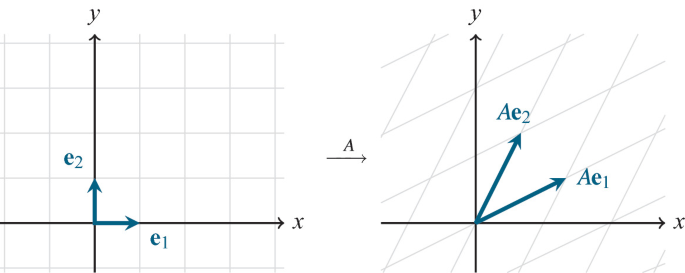
\includegraphics[width=0.75\linewidth]{chapters/chapter 4/viz Av.png}
\end{figure}


Տեսնենք, թե այն ո՞ւր է տանում ստանդարտ հենքի $\ve_1=\begin{bmatrix}
    1 \\ 0
\end{bmatrix}$, $\ve_2=\begin{bmatrix}
    0 \\ 1
\end{bmatrix}$ վեկտորները։

\[
A\ve_1 = \begin{bmatrix}
    2&1\\1&2
\end{bmatrix}\begin{bmatrix}
    1 \\ 0
\end{bmatrix}
=\begin{bmatrix}
    2 \\ 1
\end{bmatrix}
\]
\[
A\ve_2 = \begin{bmatrix}
    2&1\\1&2
\end{bmatrix}\begin{bmatrix}
    0 \\ 1
\end{bmatrix}
=\begin{bmatrix}
    1 \\ 2
\end{bmatrix}
\]

Նկատեցի՞ք․ մատրիցը հենքի $\ve_1$, $\ve_2$ վեկտորները ձևափոխելով տարավ դեպի \textit{իր իսկ սյուները՝}
\[
\begin{bmatrix}
    1 \\ 0
\end{bmatrix} \; \mapsto \; A\text{-ի } 1\text{-ին սյունը}
\]
\[
\begin{bmatrix}
    0 \\ 1
\end{bmatrix} \; \mapsto \; A\text{-ի } 2\text{-րդ սյունը}
\]

Հետևաբար եթե վերցնենք որևէ կամայական $\begin{bmatrix}
    a\\b
\end{bmatrix}$ վեկտոր՝
\begin{align*}
&\begin{bmatrix}a \\ b\end{bmatrix} = a\cdot 
\begin{bmatrix}1 \\ 0\end{bmatrix} + 
b\cdot \begin{bmatrix}0 \\ 1\end{bmatrix} \\
& \qquad \downarrow \qquad \downarrow \qquad  \downarrow \qquad \\
A&\begin{bmatrix}a \\ b\end{bmatrix} = a\cdot 
\begin{bmatrix}2 \\ 1\end{bmatrix} + 
b\cdot \begin{bmatrix}1 \\ 2\end{bmatrix} 
\end{align*}
այն կգնա դեպի նույն գործակիցներով, բայց արդեն $\ve_1$, $\ve_2$-ի փոխարեն՝ $A$-ի առաջին ու երկրորդ սյուներով վեկտորին։ 

Ավելի պատկերավոր ասած՝ բոլոր վեկտորները կառուցված են հենքի վեկտորներից․ 
\begin{itemize}
    \item երկու անգամ ձգենք $\ve_1$-ը՝ ամեն վեկտոր հորիզոնական ուղղու\-թյամբ երկու անգամ կձգվի
    \item վեց անգամ սեղմենք $\ve_2$-ը՝ ամեն վեկտոր ուղղաձիգ ուղղությամբ կսեղմվի
    \item շեղենք $\ve_2$-ը փոքր-ինչ աջ՝ բոլոր վեկտորները համապատասխան չափով կշեղվեն դեպի աջ
\end{itemize}
և այդպես շարունակ։ Ամեն ինչ կարծես կապված է հենքի վեկտորներին․ մատրիցը հենքի վեկտորները պտտելով-ձգելով տանում է իր սյուներին, արդյունքում՝ մյուս բոլոր վեկտորները նույն ձևով պտտվում-ձգվում են։

\question{$A$ մատրիցը $\ve_1$-ը սեղմում է $2$ անգամ, իսկ $\ve_2$-ը տանում է $[0 \quad -3]$ վեկտորին։ Ի՞նչ է լինում $[10 \quad 15]$ վեկտորի հետ։}

Մատրիցների վերաբերյալ խնդիրներ լուծելիս (կամ երբ ուզում եք պարզել, թե ուր է գնում այս կամ այն վեկտորը)\marginnote[*+1]{$2$-չափ կամ $3$-չափ դեպքերում} օգտակար է նայել մատրիցի սյուներին, մտքում պատկերել, թե ինչպես են $\ve_1$ և $\ve_2$ վեկտորները շարժվում դեպի մատրիցի $1$-ին ու $2$-րդ սյուները, և այդպիսով մոտավոր (ոչ շատ ճշգրիտ) պատկերացում կազմել, թե ուր է գնում Ձեր ուզած վեկտորը։

Ամփոփելով՝ արձանագրենք, որ եթե $n\times n$ չափանի $A$ մատրիցի սյուները/տողերը գծորեն անկախ են\marginnote{ասել է թե՝ $A$-ի սյուները $\R^n$-ի հենք են}, ապա այն կիրառելիս կարծես հին՝ $\ve_1$, $\dots$, $\ve_n$ հենքը փոխարինվում է նոր հենքով՝ մատրիցի սյուներով։


\begin{definition}
\marginnote{գծորեն անկախ սյուների և տողերի թիվը համընկնում է}$A$ մատրիցի գծորեն անկախ սյուների/տողերի թիվը կոչվում է $A$ մատրիցի \textbf{ռանգ։}
\end{definition}


\section{Սեփական արժեք և վեկտոր}

Երբեմն դժվար է առանց հաշվարկների ու գործիքների պատկերացնել, թե ինչպես է տրված գծային ձևափոխությունը փոխում այս կամ այն վեկտորը, հատկապես եթե ձևափոխությունը և՛ պտտում, և՛ սեղմում, և՛ ձգում է տարածությունը տարբեր ուղղություններով։ 

Օրինակ՝ \hyperref[matrix_A]{\color{OliveGreen} նախորդ բաժնից} 
\[
A = \begin{bmatrix}
    2 & 1 \\ 1 & 2
\end{bmatrix}
\]
գծային ձևափոխությունը հենքի վեկտորները մի փոքր ձգում է և պտտում՝ $\ve_1$-ը ժամսլաքի ուղղությամբ, $\ve_2$-ը՝ ժամսլաքին հակառակ։ Արդյունքում $x$-երի և $y$-երի առանցքները \marginnote{պատկերացրեք՝ ասես $x$-երի ու $y$-ների առանցքները մկրատի պոչեր են} որոշ չափով ձգվում են և մոտենում իրար․ դրանց կազմած անկյունը փոքրանում է։ 

Արդյունքում ո՞ւր է գնում, ասենք, $\begin{bmatrix}
    -3 \\ 4
\end{bmatrix}$ վեկտորը՝
\[
A\begin{bmatrix}
    -3 \\ 4
\end{bmatrix} = \begin{bmatrix}
    2 & 1 \\ 1 & 2
\end{bmatrix}\begin{bmatrix}
    -3 \\ 4
\end{bmatrix} = \begin{bmatrix}
    -2 \\ 5
\end{bmatrix}
\]

$A$-ն այն և պտտում է, և ձգում տարբեր ուղղություններով, արդյունքում՝ դժվար է առանց հաշվելու միանգամից կռահել, թե $A$-ն կիրառելիս որտեղ է այն գնում։ 

\begin{figure}[h]
    \centering
    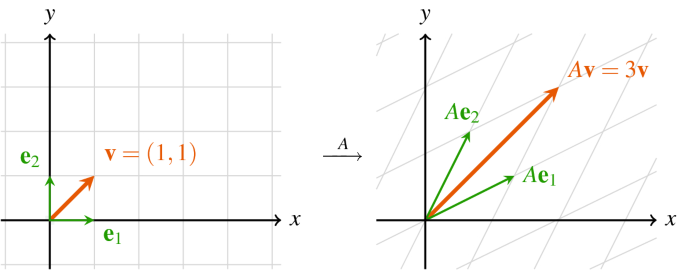
\includegraphics[width=0.75\linewidth]{chapters/chapter 4/viz eig.png}
    \caption*{$\vv$-ն մկրատի «կիսորդն» է}
\end{figure}

Մինչդեռ փոխարենը, եթե $A$-ն ընդամենը որևէ ֆիքսված չափով ձգեր կամ սեղմեր վեկտորը (ասենք՝ $3$ անգամ ձգեր), դա պատկերացնելը շատ ավելի հեշտ կլիներ։ Վերցնենք օրինակ $\vv = \begin{bmatrix}
        1 \\ 1
    \end{bmatrix}$ վեկտորը՝

\[
A \vv = \begin{bmatrix}
    2 & 1 \\ 1 & 2
\end{bmatrix}\begin{bmatrix}
    1 \\ 1
\end{bmatrix} = \begin{bmatrix}
    3 \\ 3
\end{bmatrix} = 3\cdot \begin{bmatrix}
    1 \\ 1
\end{bmatrix} = 3\vv
\]

Օ՜, հրաշք․ ստացանք նույն $\vv$ վեկտորը՝ $3$ անգամ ձգած, ու ոչ մի պտույտ կամ շրջում։

\question{Ինչպե՞ս կփոխվի $\vv$-ի կրկնապատիկը։ Իսկ $-5\vv$՞-ն։}

Առաջին վեկտորի դեպքում դժվար էր պատկերացնել, թե այն ուր է գնում, իսկ այ $\vv$-ի դեպքում ամեն բան ավելի հեշտ է, քանի որ ձևափոխության արդյունքում այն չի պտտվում, այլ մնալով նույն ուղղի վրա՝ պարզապես մի քանի անգամ ձգվում է կամ սեղմվում։ 

Այդպիսի վեկտորների հետ աշխատելը, իհարկե, շատ ավելի հեշտ է ու նախընտրելի։ Դրանք ունեն հատուկ անուն և կոչվում են գծային ձևափոխության/մատրիցի \textit{սեփական} \marginnote{$3$-ը $A$-ի սեփական արժեք է}վեկտորներ, իսկ դրանց ձգման/\linebreak սեղմման գործակիցները՝ \textit{սեփական} արժեքներ։

\begin{definition}
Եթե որևէ $\lambda$ թվի և $\vv$ ոչ զրոյական վեկտորի համար
\[
A\vv=\lambda\vv
\]
ապա կասենք, որ \marginnote{անգլերեն՝ {\it eigenvalue} և {\it eigenvector}}
\begin{itemize}
    \item $\lambda$-ն $A$-ի \textbf{սեփական արժեք} է
    \item $\vv$-ն $\lambda$-ին համապատասխան \textbf{սեփական վեկտոր} է
\end{itemize}
\end{definition}


\begin{example}
\[
A = \begin{bmatrix}
 3 & 5 \\ 1 & -1   
\end{bmatrix}
\]
գծային ձևափոխությունը  $\vv = \begin{bmatrix}
5 \\ 1
\end{bmatrix}$ վեկտորը ձգում է $4$ անգամ՝
\[A\vv =  
\begin{bmatrix}
3 & 5 \\ 1 & -1 
\end{bmatrix}
\begin{bmatrix}
5 \\ 1
\end{bmatrix}
=
\begin{bmatrix}
20 \\ 4
\end{bmatrix}
=4\vv
\]
հետևաբար $\lambda = 4$-ը $A$-ի սեփական արժեք է, իսկ $\vv$-ն՝ սեփական վեկտոր։ 
\end{example}

Եթե $A\vv=\lambda \vv$, ապա $\vv$-ի փոխարեն տեղադրելով $3\vv$, $-3\vv$, և այլն՝ ստանում ենք, որ $\vv$-ի հետ նույն ուղղի վրա ընկած ցանկացած վեկտոր նույնպես $A$-ի սեփական վեկտոր է ($\lambda$ սեփական արժեքին համապատասխան)։ 
\begin{theorem}
Եթե $\vv$-ն $A$-ի սեփական վեկտոր է, ապա $c\vv$-ն ևս $A$-ի սեփական վեկտոր\marginnote{նույն արժեքին համապատասխան} է (ցանկացած $c\ne 0$ թվի համար)։
\end{theorem}

Ուրեմն եթե $\lambda$ թիվը $A$-ի սեփական արժեք է, ապա $A$-ն ոչ թե ունի մեկ-երկու վեկտոր, այլ ամբողջական \textit{ուղղություններ,} որոնց վրա կիրառելիս դրանք պարզապես $\lambda$ անգամ ձգում է։ 

\question{Կարո՞ղ է $\vv$ վեկտորը համապատասխանել երկու տարբեր $\lambda_1$ և $\lambda_2$ սեփական արժեքների։}

$A$-ի բոլոր սեփական արժեքների բազմությունը անվանում են $A$-ի \textit{սպեկտր,} իսկ յուրաքանչյուր $\lambda$ սեփական արժեքին համապատասխանող սեփական վեկտորների բազմությունը՝ $\lambda$-ին համապատասխան \textit{սեփա\-կան տարածություն}\marginnote{անգլերեն՝ {\it eigenspace}} (նշանակում են՝ $E_\lambda$):

\warning{$n\times n$ չափանի մատրիցը ամենաշատը կարող է ունենալ $n$ սեփական արժեքներ, կարող է նաև ընդհանրապես չունենալ։}

\question{Կարո՞ղ եք նկարագրել $\R^2$-ի այնպիսի ձևափոխություն, որը սեփական արժեք չունի։ Իսկ այնպիսին, որն ունի ուղիղ մեկը՞։}

Ինչպե՞ս մատրիցի հետ թվաբանական գործողություններ անելով գտնենք նրա սեփական արժեքները։ Եկեք պարզենք դա՝ առանց հաշվողական մասի վրա խորանալու։ Ուզում ենք գտնել այնպիսի $\lambda$ և $\vv$, որ $A\vv= \lambda \vv$։ Նշանակենք $\lambda$-ն $x$-ով և գրենք՝
\[
A\vv= x \vv = x(I\vv) = (xI)\vv
\]
կամ որ նույնն\marginnote{ի՞նչ տեսք ունի $xI$ մատրիցը} է՝ $A\vv-(xI)\vv = (A-xI)\vv= \mathbf{0}$:

Եթե $(A-xI)$ մատրիցը ունենար հակադարձ, կգրեինք՝
\[
\vv = (A-xI)^{-1}\mathbf{0}
\]
բայց ցանկացած մատրիցի և $\mathbf{0}$-ի արտադրյալը հենց $\mathbf{0}$ է, ուրեմն կստացվեր $\vv = \mathbf{0}$, բայց չէ՞ որ պահանջել էինք, որ սեփական վեկտորը զրոյական չլինի։ Հետևաբար $(A-xI)$-ն հակադարձ չունի՝
\[
\det(A-xI)=0
\]

Ահա այս հավասարման ձախ մասում գրվածը որոշիչի բանաձևով կբացենք, կստանանք $x$-ից կախված մի բազմանդամ (կոչվում է՝ $A$-ի \textit{բնութագրիչ բազմանդամ}), և եթե գտնենք դրա արմատները՝ ստացված թվերը կլինեն $A$-ի սեփական արժեքները։ Խնդրի լուծման կոնկրետ օրինակ կարող եք տեսնել օրինակ՝ \href{https://www.youtu.be/UVZ4kStUo1s}{այստեղ}, սակայն ինչպես մեծ չափանի մատրիցների որոշիչի, այնպես էլ սեփական արժեքների դեպքում՝ ձեռքով դրանց հաշվելը երկար գործ է, ուստի մենք դրա վրա չենք կենտրոնանա։

Փոխարենը, հետևյալ գեղեցիկ հատկությունները կապ են հաստատում գծային ձևափոխության երեք տարբեր բնութագրիչների՝ սեփական արժեքների, որոշիչի և հետքի միջև․
\begin{theorem}
Քառակուսային մատրիցի որոշիչը հավասար է նրա սեփական արժեքների արտադրյալին․
\[
\det(A) = \lambda_1 \cdot \lambda_2 \cdot \ldots \cdot \lambda_n
\]
իսկ \marginnote{սիրուն է, չէ՞} հետքը՝ սեփական արժեքների գումարին․
\[
\operatorname{tr}(A) = \lambda_1 + \lambda_2 + \ldots + \lambda_n
\]
\end{theorem}



\bigskip 

\begin{theory}
.
\begin{itemize}
\item կարդալ [{\rm Johnston}], 126-129 (գծային թաղանթ), 131-135 (գծորեն անկախություն), 140-141 (հենք) էջերը  
\item դիտել  {\rm 3b1b}-ի \href{https://www.3blue1brown.com/lessons/span}{2-րդ} տեսադասը գծային հանրահաշվից 
\item կարդալ [{\rm Poole}], 202-203 էջերը (չափողականություն)
\item վերադառնալ [{\rm Johnston}], 38-41 և 235-237 (մատրիցի սյունե\-րի և հենքի կապը), 285-286 (սեփական արժեքներ) էջերին
\item ըստ ցանկության՝ [{\rm Poole}], 255-259 էջերի օրինակներին
\item դիտել {\rm 3b1b}-ի \href{https://www.3blue1brown.com/lessons/eigenvalues}{14-րդ} տեսադասը գծային հանրահաշվից 
\item տեսնել սեփական վեկտորները \href{https://setosa.io/ev/eigenvectors-and-eigenvalues}{սեփական աչքով}
\item ըստ ցանկության՝ հետազոտել \href{https://www.youtu.be/mhy-ZKSARxI}{սեփական արժեքներով} և \href{https://www.ams.org/publicoutreach/feature-column/fcarc-svd}{եզակի արժեքներով} մատրիցի վերլուծության մասին
\end{itemize}
\end{theory}

\newpage

\section{Խնդիրներ}


\begin{problem}\marginnote[*+0.5]{\href{https://youtu.be/5VEnDdm8RZo}{լուծում}}
Լրացրեք բացակայող թվերը՝
\[
\begin{bmatrix}
    2 & * \\ -1 & *
\end{bmatrix}
\]
եթե հայտնի է, որ
\begin{enumerate}[label={\alph*}․]
\item ձևափոխությունը ձգում է $\begin{bmatrix}
    1 & 0
\end{bmatrix}$ վեկտորը $2$ անգամ

\item ձևափոխությունը հետքը $2$ է, իսկ որոշիչը՝ $3$

\item $1$-ն ու $5$-ը ձևափոխության սեփական արժեքներ են
\end{enumerate}

\end{problem}

\begin{problem}
Ամենաշատը ի՞նչ չափողականության ենթատարածություն է կարելի կառուցել այս վեկտորներով․
\begin{enumerate}[label={\alph*}․]
\item $\vv_1=\begin{bmatrix}6\\1\\5\end{bmatrix}$,  $\vv_2=\begin{bmatrix}
    2\\3\\2
\end{bmatrix}$

\item $\vv_1=\begin{bmatrix}6\\2\end{bmatrix}$,  $\vv_2=\begin{bmatrix}
    1\\3
\end{bmatrix}$,  $\vv_3=\begin{bmatrix}
    5\\2
\end{bmatrix}$

\item $\vv_1=\begin{bmatrix}4\\1\\2\end{bmatrix}$,  $\vv_2=\begin{bmatrix}
    -4\\2\\-1
\end{bmatrix}$,  $\vv_3=\begin{bmatrix}
    8\\-1\\7
\end{bmatrix}$

\item $\vv_1=\begin{bmatrix}3\\-2\\1\end{bmatrix}$, $ \vv_2=\begin{bmatrix}
    6\\-4\\4
\end{bmatrix}$
\end{enumerate}
\end{problem}


\begin{problem}
Գտեք հետևյալ ձևափոխությունների սեփական արժեքներն ու վեկտորները․

\begin{enumerate}[label={\alph*}․]
\item $A=\begin{bmatrix}
    1&2\\0&1\end{bmatrix}$

\item $B=\begin{bmatrix}
    2&1\\1&2
\end{bmatrix}$

\item $C=\begin{bmatrix}
    8 & 1 \\ 8 & 1
\end{bmatrix}$

\item $D=\begin{bmatrix}
-1&0&0\\0&1&0\\0&0&3        \end{bmatrix}$
\end{enumerate}

Կարող եք օգտվել մեր իմացած ցանկացած մեթոդից (բնութագրիչ բազմանդամ, հետք և որոշիչ, սյուների ու հենքի կապը), բայց փորձեք նաև տեսողաբար պատկերացնել խնդիրը։
\end{problem}



\begin{problem}
Ենթադրենք ունենք
\[
A=\begin{bmatrix}
    a_1 & 0 & 0 & 0 & 0 \\
    0 & a_2 & 0 & 0 & 0 \\
    0 & 0 & a_3 & 0 & 0 \\
    0 & 0 & 0 & a_4 & 0 \\
    0 & 0 & 0 & 0 & a_5 
\end{bmatrix}
\]
գծային ձևափոխությունը, որտեղ $a_1, \dots, a_5$-ը որևէ ֆիքսված դրական թվեր են։
\begin{enumerate}[label={\alph*}․]
\item ո՞րն է $\mathbb{R}^5$ տարածության ստանդարտ հենքը

\item ո՞ւր է տանում $A$-ն $\mathbb{R}^5$-ի ստանդարտ հենքի վեկտորներին

\item ի՞նչ եք կարծում, որքա՞ն է $A$-ի որոշիչը

\item կարո՞ղ եք գտնել $A$-ի սեփական արժեքներն ու վեկտորները
\end{enumerate}


\end{problem}


\begin{problem}
Ֆեյսբուքում հանդիպելով հետևյալ խնդրին՝
\begin{quote}
\textit{$2$ խնձորն ու $3$ տանձը միասին արժեն $1100$ դրամ, իսկ $1$ խնձորն ու $4$ տանձը՝ $700$ դրամ։ Միայն $140$-ից բարձր {\it IQ} ունեցող մարդիկ կարող են գտնել խնձորի ու տանձի գինը։}
\end{quote}
հասկանում եք, որ եկել է պահը՝ վերջապես կիրառելու Ձեր սովորածը։
\begin{enumerate}[label={\alph*}․]
\item անհայտները նշանակելով $x_1$, $x_2$-ով՝ գրեք խնդիրը համակարգի տեսքով

\item կարո՞ղ եք պայմանները արտահայտել
\[
\begin{bmatrix}
    * & * \\ * & *
\end{bmatrix}\begin{bmatrix}
    x_1 \\ x_2
\end{bmatrix}
= \begin{bmatrix}
    * \\ *
\end{bmatrix}
\]
տեսքով, կարճ՝ $A\vx = \vb$

\item օգտվելով հակադարձի բանաձևից՝ փորձեք գտնել $\vx$-ը
\end{enumerate}

Այն, ինչ ստացաք, կոչվում է \textit{գծային հավասարումների համակարգ։}

\end{problem}
